% Szglab4
% ===========================================================================
%
\setcounter{chapter}{-1}

\chapter{Módosítások}

\subsection{Bemeneti nyelv}

\begin{itemize}
	
\item Cleaner <x> <y>
    \begin{itemize}
	\item Leírás: Cleaner létrehozása a pályán megadott koordinátákon.
	\item Opciók: Két koordináta.
	\end{itemize}
	
\item cycles\_elapsed <amount> 
	\begin{itemize}
	\item Leírás: Szimulálja, hogy hányat léptek a robotok a játékon belül.
	\item Opciók: Lépésszám megadása.
	\end{itemize}

\item Glue <x> <y>
	\begin{itemize}
	\item Leírás: Ragacs létrehozása a pályán.
	\item Opciók: A ragacs (x,y) koordinátái.
	\end{itemize}
	
\item keyPressed <akadály\_gomb>
	\begin{itemize}
	\item Leírás: Akadály lerakása a robot koordinátáira.
	\item Opciók: 
	\begin{itemize}
    	    \item akadály\_gomb
        	    \begin{itemize}
        	        \item Up: Robot1 olaj lerakás
        	        \item Down: Robot1 ragacs lerakás
        	        \item W: Robot2 olaj lerakás
        	        \item S: Robot2 ragacs lerakás
        	    \end{itemize}
    	\end{itemize}
	\end{itemize}
	
\item keyPressed <irány\_gomb> <forgás értéke fokban>
	\begin{itemize}
	\item Leírás: A Robot következő irányának változtatása.
	\item Opciók: 
    	\begin{itemize}
    	    \item irány\_gomb
        	    \begin{itemize}
        	        \item Left: Robot1 balra forgatása
        	        \item Right: Robot1 jobbra forgatása
        	        \item A: Robot2 balra forgatása
        	        \item D: Robot2 jobbra forgatása
        	    \end{itemize}
        	 \item forgás érték = (0,180)
    	\end{itemize}
	\end{itemize}
	
\item listCleaners
	\begin{itemize}
	\item Leírás: A palyán lévő takarító kisrobotok kilistázása.
	\item Opciók: -
	\end{itemize}
	
\item listObstacles
	\begin{itemize}
	\item Leírás: Kilistázza a pályán lévő akadályokat.
	\item Opciók: -
	\end{itemize}
	
\item listRobots
	\begin{itemize}
	\item Leírás: Kilistázza a robotokat.
	\item Opciók: -
	\end{itemize}
	
\item MapBuilder 
	\begin{itemize}
	\item Leírás: Pálya betöltése a játékba.
	\item Opciók: Pálya kiválasztása.
	\end{itemize}	
	
\item move
	\begin{itemize}
	\item Leírás: Robotok, Cleanerek mozgatása.
	\item Opciók: -
	\end{itemize}
	
\item Oil <x> <y>
	\begin{itemize}
	\item Leírás: Olajfolt létrehozása a pályán.
	\item Opciók: Az olajfolt (x,y) koordinátái.
	\end{itemize}

\item Phoebe <mode> <count>
	\begin{itemize}
	\item Leírás:\\ Egy teljes értékű játék indítására való parancs. Inicializál két robotot és pár Obstaclet. A játék indulásához szükséges feltételek teszteléséhez szolgáló parancs.
	\item Opciók:
		\begin{itemize}
			\item mode
			\begin{itemize}
				\item time: Időjátékmódú menet beállítás
				\item lap: Körjátékmódú menet beállítása
			\end{itemize}
			\item count: 
			\begin{itemize}
				\item Időjátékmód esetén a rendelkezésre álló időt kell megadni másodpercben.
				\item Körjátékmód esetén a teljesítendő körök számát kell megadni.
			\end{itemize}
		\end{itemize}
	\end{itemize}

\item Robot <x> <y>
    \begin{itemize}
	\item Leírás: Robot létrehozása a pályán megadott koordinátákon.
	\item Opciók: Két koordináta.
	\end{itemize}
	
\item setCheckpoints
	\begin{itemize}
	\item Leírás: A pálya checkpointjainak a beállítása.
	\item Opciók: -
	\end{itemize}
	
%\item time\_spend <count>
%	\begin{itemize}
%	\item Leírás:\\ A játékban nagy szerepet játszik az idő múlása. Ezzel a paranccsal a tesztelő szimulálhatja, hogy bizonyos másodperccel előrelépjen a játék a működésében. Ekkor nem gyorsul fel a játék, csak az órát pörgetjük tovább.
%	\item Opciók:\\
%		\begin{itemize}
%			\item count: Az eltelendő idő megadása másodpercben.
%		\end{itemize}
%	\end{itemize}
%\end{itemize}

	
	
	\item  time\_spend <count>
	\begin{itemize}
	\item Leírás: A játékban nagy szerepet játszik az idő múlása. Ezzel a paranccsal a tesztelő szimulálhatja, hogy bizonyos másodperccel előrelépjen a játék a működésében. Ekkor nem gyorsul fel a játék, csak az órát pörgetjük tovább.
	\item Opciók: Az eltelendő idő megadása másodpercben.
	\end{itemize}	
\end{itemize}

\chapter{Részletes tervek}

\thispagestyle{fancy}

\section{Osztályok és metódusok tervei}

\section{Objektum katalógus}

\subsection{Glue}
A „Glue” objektum megvalósít egy adott tulajdonságú akadályt. Amely robot belemegy, annak a sebességét megfelezi. 
\subsection{GUI}
A grafikus felületet megvalósító objektum. Ez az objektum maga a menü, ami a játék indítása után ugrik fel. Itt találhatóak a beállítások (mint például a gondolkodás idő és a maximális játék idő vagy a körök száma) és a játékmódok. Gombnyomásra fogja elindítani a játék működési szálát. Ez az objektum kezeli az ablak eseményeit és a játék bezárását.
\subsection{HUD}
Ez az objektum követi és nyilvántartja, hogy a robotok hány checkpoint-on mentek át, illetve kiírja a képernyőre a hátramaradó időt és a megtett körök számát. Feladata, hogy minden körben megvizsgálja, hogy a robotok elérték-e a következő checkpointot.
\subsection{MapBuilder}
Fájlból beolvassa és létrehozza a memóriában a pályát, a kezdő pozíciókat és a checkpointokat reprezentáló objektumokat.  Mivel a  MapBuilder objektum tárolja a pályát így feladat, hogy vizsgálja a robotok, akadályok azon belül tartózkodását.  
\subsection{Oil}
Ez az objektum az Obstacle osztály leszármazottja. Hasonlóan a Glue objektumhoz, egy adott hatást valósít meg, ami letiltja a következő körben történő irányítását a robotnak, ami belelépett.
\subsection{Phoebe}
A játék logikát megvalósító objektum. Listában tárolja a pályán tartózkodó robotokat, akadályokat és figyeli, hogy mikor ér véget a játék. A „Phoebe” objektum rajzolja ki az objektumokat a pályán és szálként indítható osztályt, melyben maga a játék fut. Játékindításkor berakja a pályára a robotokat és az akadályokat a kezdő pozíciókba. Ebben az objektumban történnek az ellenőrzések (akadályba vagy robotba ütközések, pályáról leesés).
\subsection{Robot}
Olyan objektum, mely a pályán található robotokat valósítja meg. Leírja a viselkedésüket és a kezelésüket. A „Robot” osztály a Unit-ból származik le, ezáltal van pozíciója és az ütközés is le van kezelve. Felelős a mozgásért, megállapítja egy adott akadállyal vagy robottal ütközött-e és kezeli a robot által felhasználható akadálykészleteket, illetve tartalmaz gombnyomást lekezelő metódusokat is.
\subsection{MyTimer}
Az eltelt időt és a fennmaradt idő nyilvántartásáért felelős. Ilyen például a játék elején a három másodperces visszaszámlálás vagy az időlimites játékmód esetén, amikor a maximális időtől számol visszafelé.

\subsection{MyListener}
A játék keylistener-jét megvalosító osztály. Külön szálon fut, hogy az egyszerre lenyomott gombok ne okozhasanak problémát. A játékban részvevő robotok KeyPressed függvényét hivogatja, a megfelelő KeyEvent paraméterrel.
\subsection{Cleaner}
Takarító robotk melyek a pályán olaj és ragacsfoltokat szednek fel. A robotkkal való ütközés során megsemmisülhetnek.
\pagebreak
\section{Statikus struktúra diagramok}

\begin{figure}[h]
\begin{center}
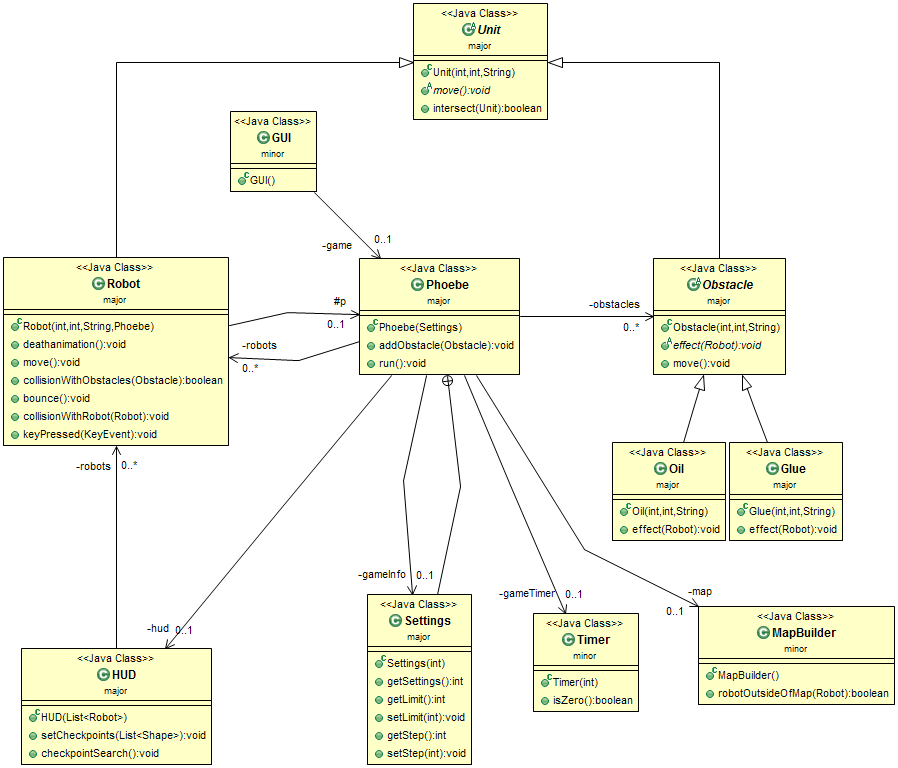
\includegraphics[width=17cm]{images/struktdiagram.PNG}
\caption{Osztály diagram}
\label{fig:example3}
\end{center}
\end{figure}


\section{Osztályok leírása}

\subsection{Cleaner}
\begin{itemize}
\item Felelősség\\
A takarító robotot reprezentáló osztály.
\item Ősosztályok\\
Unit$\rightarrow$Robot
\item Attribútumok
    \begin{itemize}
        \item List obstacles:  
    \end{itemize}
\item Metódusok
	\begin{itemize}
	    \item \textbf{Cleaner}(int x, int y, Phoebe p):
		\item void \textbf{setObstacles}(List obsts): 
		\item boolean \textbf{collisionWithRobot}():
		\item void \textbf{collisionWithCleaner}():
		\item void \textbf{move}():
	\end{itemize}
\end{itemize}



\subsection{GUI}
\begin{itemize}
\item Felelősség\\
A grafikus felületért felelős osztály, amely a menüt és a játékot jeleníti meg.
\item Attribútumok
	\begin{itemize}
		\item \textbf{Phoebe} game: referencia a játékra
	\end{itemize}
\item Metódusok
	\begin{itemize}
		\item\textbf{GUI}(): Konstruktor. Beállítja az ablak nevét, létrehozza az ablak elemeit, elrendezi őket és beállítja a figyelőket(ActionListener).
	\end{itemize}
\end{itemize}

\subsection{HUD}
\begin{itemize}
\item Felelősség\\
A robotok megtett köreit és checkpontjait tartja számon. Megvalósítja a checkpoint ellenőrzést.
\item Attribútumok
	\begin{itemize}
		\item \textbf{int[]} checkpointReached: Minden robothoz külön tárolja a legutoljára érintett checkpoint sorszámát.
		\item \textbf{int[]} lap: Minden robothoz tárolja a megtett körök számát. 
		\item \textbf{List} checkpoints: Tárolja a checkpointokat reprezentáló objektumokat List adatszerkezetben. A checkpointSearch függvény kérdezi le ebből a következő checkpoint helyzetét. 
		\item \textbf{List<Robot>} robots: A robotokat tároló List adatszerkezet. A checkpointSearch függvény kérdezi le ebből a robotokat, majd azok helyzetét.
	\end{itemize}
\item Metódusok
	\begin{itemize}
		\item \textbf{HUD}(List<Robot> robs): Robot objektumokat tároló ArrayList. Célja, hogy a checkpointsearch() függvényben minden robotra elvégezzük a keresést.
		\item void \textbf{checkpointSearch}(): Minden híváskor ellenőrzi, hogy a robot és a checkpoint metszete üres-e. 
		\item int \textbf{endOfTheGame}(): A játék végén eldönti, hogy melyik játékos nyert. Visszatér egy számmal, amiből egyértelműen eldönthető, hogy ki nyert. Ha negatív akkor az 1-es számú játékos nyert, ha nulla akkor döntetlen, ha pozitív akkor a 2-es számú játékos nyert.
		\item void \textbf{setCheckpointReached}(Robot r): Ha a paraméterként átadott robot következő checkpointja a célvonal (utolsó checkpoint) akkor lenullázza a checkpointReached-et és növeli a megtett körök számát, illetve ha nem akkor növeli az érintett checkpointok számát.
		\item void \textbf{setCheckpoints}(List checkObj): Checkpointokat reprezentáló adatszerkezet betöltése.CheckpointReached inicializálása a checkpointok számától függően.
	\end{itemize}
\end{itemize}

\subsection{IVisible}
\begin{itemize}
\item Felelősség\\
A grafikus motorhoz szükséges interfész. Olyan osztályok, melyek kirajzolható elemeket tartalmaznak megvalósítják ezt az interfészt.
\item Metódusok
	\begin{itemize}
		\item void \textbf{paint}(Graphics2D g): Rajzolást elvégző metódus.
	\end{itemize}
\end{itemize}

\subsection{List}
\begin{itemize}
    \item Felelősség
        \begin{itemize}
        \item Objektumok tárolása, ezt az interfészt megvalósító osztályban.
        \item \url{https://docs.oracle.com/javase/6/docs/api/java/util/List.html}
        \end{itemize}
\end{itemize}

\subsection{MapBuilder}
\begin{itemize}
\item Felelősség\\
A pálya felépítéséért, a checkpointok tárolásáért és a robot pályán tartózkodásának vizsgálatáért felelős osztály.
\item Attribútumok
	\begin{itemize}
		\item \textbf{List} checkpoints: Tárolja a checkpointokat reprezentáló objektumokat List adatszerkezetben.
		\item \textbf{Object} map: A pályát reprezentáló objektum.
		\item \textbf{int[]} startPosPlayerOne: Meghatároz egy (x,y) koordinátát, ahol az első játékos kezd.
		\item \textbf{int[]} startPosPlayerTwo: Meghatároz egy (x,y) koordinátát, ahol az második játékos kezd.
	\end{itemize}
\item Metódusok
	\begin{itemize}
		\item \textbf{MapBuilder}(): Konstruktor, a pálya beolvasása fájlból, majd létrehozása.
		\item int[] \textbf{getStartPosPlayer}(int id): Paraméterül kap egy Robot id-t, majd visszatér egy int tömbbel, melyben található a robot kezdőpozíciója a pályán.
		 \item boolean \textbf{obstacleOutsideOfMap}(Obstacle obs): Egy akadályt vizsgál, hogy a pályán van-e.
		\item boolean \textbf{robotOutsideOfMap}(Robot r): Igaz értéket ad vissza, ha a robot leesett a pályáról, hamisat ha még rajta van.
	\end{itemize}
\end{itemize}

\subsection{MyListener}
\begin{itemize}
\item Felelősség\\
A külön szálon futó KeyListener-t megvalósító osztály.
\item Interface-ek:
    \begin{itemize}
    \item KeyListener
    \item Runnable
    \end{itemize}
\item Attribútumok
	\begin{itemize}
		\item -\textbf{boolean} isUp: Azt tárolja, hogy le van-e nyomva a felfele nyil.
    	\item -\textbf{boolean} isDown: Azt tárolja, hogy le van-e nyomva a lefele nyil.
    	\item -\textbf{boolean} isRight:Azt tárolja, hogy le van-e nyomva a jobbra nyil.
    	\item -\textbf{boolean} isLeft:Azt tárolja, hogy le van-e nyomva a balra nyil.
    	\item -\textbf{boolean} isW:Azt tárolja, hogy le van-e nyomva a W a billentyűzeten.
    	\item -\textbf{boolean} isD:Azt tárolja, hogy le van-e nyomva a D a billentyűzeten.
    	\item -\textbf{boolean} isS:Azt tárolja, hogy le van-e nyomva az S a billentyűzeten.
    	\item -\textbf{boolean} isA:Azt tárolja, hogy le van-e nyomva az A a billentyűzeten.
   	\item -\textbf{List<Robot>} robots: Azon robotok listája akiknek a keyPressed függvényét kell hívnia.
	
	
	\end{itemize}
\item Metódusok
	\begin{itemize}
		\item+ \textbf{MyListener}(List<Robot> r): beállítja a lenyomott gombokat figyelő változókat false-ra , továbbá beállítja a robots változó referenciáját a paraméterként kapotra.
			\item+ void\textbf{keyPressed}(KeyEvent e): Beállítja a lenyomot gombokat figyelő változók küzül a Keyeventnek megfelelőt  true-ra , ha meg nyomták valamelyiket  a figyelt gombok közül.
			\item+ void\textbf{keyReleased}(KeyEvent e): Beállítja a lenyomot gombokat figyelő változók küzül a Keyeventnek megfelelőt false-ra , ha fel engedték valamelyiket a figyelt, lenyomott gombok közül.
				\item+ void\textbf{run}(): Végtelen ciklust futtat. Megvizsgálja hogy melyik gombok vannak lenyomva, majd a nekik megfelelő KeyEvent-tel paraméterezve meghívja a hozzátartozó robotoknak a Keypressed függvényét. Majd alszik a szál 30 mili secundomig.
	\end{itemize}
\end{itemize}

\subsection{MyTimer}
\begin{itemize}
\item Felelősség\\
A játék elején a kezdésig visszaszámol három másodpercet, utána indulhat a játék. Játéktípustól függően felfelé(kör játékmód) vagy visszafelé(idő játékmód) számol. Ez az osztály felelős, azért ha lejár az idő vége legyen a játéknak,
\item Attribútumok
    \begin{itemize}
        \item - enum DIR: Az óra számolási irányának enumerizácciója.
        \item - long T\_start: Az óra indításának időpontja millisec pontosággal.
	    \item - int duration: Ha az óra visszafelé számol, akkor tárolja, hogy mennyi volt a kezdő érték, ha felfelé számol, akkor értéke 0. Mértékegysége millisekundum.
	    \item - DIR direction: Az óra számolási irányának eltárolásáért felelős enum.
    \end{itemize}
\item Metódusok
	\begin{itemize}
		\item + \textbf{MyTimer}(int i): Konstruktor. Ha 0-val vagy negatívval inicializálják felfele számol, ha pozitív számmal inicializálják akkor lefelé számol.
		\item + boolean \textbf{isZero}(): Az idő lejárását ellenörző függvény, megadja, hogy az indítás plusz a megadott időtartam kisebb-e a pillanatnyi időnél.
		\item + int \textbf{getTime}():  Ha pozitív száámal inicializálódott az objektum, akkor megadja mennyi idő van még hátra a visszaszámlálásból vagy, ha nullával, akkor a start() hívás óta eltelt idővel tér vissza.
		\item + void \textbf{start}(): Az óra indításakor vagy újraindításakor meghívott függvény. Csak akkor indul újra (visszaszámláló üzemmódban), ha elérte a 0-t. A Phoebe run() metódusa hívja meg, mikor vissza kell számolni a játék kezdete előtt három másodpercet. Illetve, a játék kezdetekor.
	\end{itemize}
\end{itemize}

\subsection{Obstacle}
\begin{itemize}
\item Felelősség\\
A pályán/játékosoknál lévő különböző akadályokat (ragacs,olaj) összefogó ősosztály.
\item Ősosztályok\\
Unit
\item Attribútumok
	\begin{itemize}
		\item \# \textbf{int} WIDTH: Az akadályokat jellemző szélesség. Szükség van rá, hogy létrehozzuk a leszármazottak hitbox-át(sokszög pályaelem).
		\item \# \textbf{int} HEIGHT: Az akadályokat jellemző hosszúság. Szükség van rá, hogy létrehozzuk a leszármazottak hitbox-át(sokszög pályaelem).
			\item \# \textbf{int} lifetime: Generikussan az akadályok életben maradásának ellenörzésére szolgál. Olaj esetében megadja, hogy hány kör telt el az akadály lerakása óta. Ragacs esetében pedig, hogy hányan léptek rá mióta lekerült. 
	\end{itemize}
\item Metódusok
	\begin{itemize}
		\item +\textbf{Obstacle}(int x, int y): meghívja a Unit konstruktorát a megadott adatokkal és létrehoz egy négyzet elemet ami reprezentálja a pályán majd.
		\item + void \textbf{effect}(Robot r): Meghatározza, milyen hatással van a robotra, ha érintkezik egy Obstacle-lel. Absztrakt.
		\item +boolean \textbf{checkAlive}():Az akadályok vizsgálata amit a játékmotor minden körben meghív minden akadályra. Absztrakt.
	\end{itemize}
\end{itemize}

\subsection{Glue}
\begin{itemize}
\item Felelősség\\
A játékban szereplő Ragacs foltok viselkedését leíró osztály
\item Ősosztályok\\
Unit$\rightarrow$Obstacle
\item Attribútumok
	\begin{itemize}
		\item -\textbf{BufferedImage} img: Ez a  statikus atribútum a ragacs képét tárolja,  a megjelenítésben van szerepe.
	\end{itemize}
\item Metódusok
	\begin{itemize}
		\item  \textbf{Glue}(int x,int y):A ragacs konstruktora, meghívja az őse (obstacles)                           konstruktorát x,y paraméterrel, továbbá beállítja a lifetime-ot 4-re.
		
		\item+ void \textbf{effect}(Robot r): Ütközéskor hívja meg az ütközést vizsgáló függvénye     a Robot osztálynak. Módosítja a robot slowed értékét a 50\%-ra a robot slowed attribútum         setterének meghívásával. Továbbá csökkenti a ragacs élettartalmát egyel.
	
		\item+ boolean \textbf{checkAlive}():A játékmotor hívja meg minden kör végén, ha a lifetime értéke>0 true-val tér vissza, különben false-al.
			\item+ void \textbf{paint}(Graphics2D g):Kirajzolja a ragacs képét az x,y koordinátákon.
				\item+ void \textbf{setUnitImage}():Beállítja a ragacs osztályhoz tartozó képet a user directoryban található glue.jpg-re
			\item+ String \textbf{toString}()Vissza ad egy stringet a  ragacs legfontosabb értékeivel.(x, y, WIDTH, HEIGHT, lifetime)
		
	\end{itemize}
\end{itemize}

\subsection{Oil}
\begin{itemize}
\item Felelősség\\
A pályára lerakható olaj megvalósítása. Ha belelép egy játékos egy ilyen olajfoltba az effect függvény letiltja a mozgatást az adott roboton a következő ugrásig.
\item Ősosztályok\\
Unit $\rightarrow$ Obstacle 
\item Attribútumok
	\begin{itemize}
		\item- \textbf{BufferedImage} img: Ez a  statikus atribútum az olaj képét tárolja,  a megjelenítésben van szerepe.
	\end{itemize}
\item Metódusok
	\begin{itemize}
		\item + \textbf{Oil}(int x, int y): Egy Oil elem létrehozásáért felelős. Meghívja az ős konstruktorát x,y-paraméterrel, továbbá beállítja a lifetime-ot default értékre.
		\item + void \textbf{effect}(Robot r): Meghatározza, milyen hatással van a robotra, ha beleugrik egy olajfoltba. Ebben az esetben letiltja a játékost, hogy irányt váltson.
			\item + void \textbf{setUnitImage}():Beállítja az olaj osztályhoz tartozó képet a user directoryban található oil.jpg-re
				\item + boolean \textbf{checkAlive}():A játékmotor hívja meg minden kör végén, lifetime értékét csökkenti 1 el, ha a lifetime értéke>0 (csökkentés után)true-val tér vissza, különben false-al.
		\item + String \textbf{toString}()Vissza ad egy stringet az olaj legfontosabb értékeivel.(x, y, WIDTH, HEIGHT, lifetime)
	\end{itemize}
\end{itemize}

\subsection{Phoebe}
\begin{itemize}
\item Felelősség\\
A játék motorját megvalósító objektum. Listában tárolja a pályán tartózkodó robotokat,kisrobotokat, akadályokat és 
 figyeli, hogy mikor ér véget a játék. A „Phoebe” objektum rajzolja ki az objektumokat a pályán és 
 szálként indítható osztályt, melyben maga a játék fut. Játékindításkor berakja a pályára a robotokat és 
 az akadályokat a kezdő pozíciókba. Ebben az objektumban történnek az ellenőrzések (akadályba vagy 
  robotba ütközések, pályáról leesés)
  \item Interface:
  \begin{itemize}
  \item Runnable
  \end{itemize}
\item Attribútumok
	\begin{itemize}
		\item- \textbf{boolean} ended: Állapot változó, ha vége a játéknak, akkor true. Ha beteljesül egy játék végét jelentő esemény, akkor ezen a változón keresztül leáll a játék és megállapítódik a nyertes.
		\item+ \textbf{BufferedImage} background: A játék hátterét adó kép.
		\item- \textbf{List<Robot>} robots: A játékban szereplő robotok listája.
		\item- \textbf{List<Obstacle>} obstacles: A játékban szereplő akadályok listája.
		\item- \textbf{HUD} hud: A játékosok előrehaladását, ragacs és olajkészleteit tartja számon
		\item- \textbf{MapBuilder} map: TODO
		\item- \textbf{Settings} gameInfo:A játék beállításait tartalmazza         \item- \textbf{List<Cleaner>} cleaners: A játékban lévő aktív kis tisztogató robotokat tartja számon.
        \item- \textbf{MyTimer} gameTimer: A játékban futó óra, ami visszaszámlálásoknál és a játék végének meghatározásánál játszik szerepet.

		
			
	\end{itemize}
\item Metódusok
	\begin{itemize}
		\item+ \textbf{Phoebe}(Setting set): A játék felépítése, a robotok,a tisztogató kisrobotok és  az akadályok listáinak létrehozása.Az ended inicializálása ,az init függvény meghívása és a grafikus felület felépítése történik itt.
		\item+ void \textbf{run}(): Ez a metódus futtatja a főciklust, amelyben maga a játék működik.
	\item+ void \textbf{Paint}(Graphics2D g2d): Kirajzolja a játék aktuális állását. 
	\item+ void \textbf{addObstacle}(Obstacle item): Hozzá ad egy Obstacle-t a játékban lévők listájához.
	
	\item- void \textbf{init}(): Inicializálja a játékot a kezdeti beállításokra. Létrehozza az időzítőt, a mapot, a robotokat a kezdőpozíciók szerint,a hudot és beállítja a különböző osztályokhoz tartozó statikus képeket, továbbá a pálya alap ragacsait és olajait is szétszórja.
	\end{itemize}
\end{itemize}

\subsection{Robot}
\begin{itemize}
\item Felelősség\\
A játékban résztvevő ugráló robotok viselkedését és kezelését leíró osztály, tárolja és kezeli a felhasználható akadályok számát.
  Olyan objektum, mely a pályán található robotokat valósítja meg. Leírja a viselkedésüket és a kezelésüket. 
  A „Robot” osztály a Unit-ból származik le, ezáltal van pozíciója és az ütközés is le van kezelve. 
  Felelős a mozgásért, megállapítja egy adott akadállyal vagy robottal ütközött-e és kezeli a felhasználó által leütött gombokat.
  \item Ősosztályok\\
Unit

\item Attribútumok
	\begin{itemize}
		\item\# \textbf{int} staticID: Az osztályhoz tartozó statikus azonosító, a példány                azonosítójának(id) meghatározásához szükséges.
			\item- \textbf{static final int} r: Az ugrás számításához tartozó sugár. 
				\item- \textbf{static final int} ANIMATIONSPEED: Az ugrás animálásának részletessége(hányszor hívja meg a paintet). 
		\item\# \textbf{static int} HEIGHT: A robot képének magassága, collision                      detektálásnál, továbbá az irányítást segítő nyíl kezdő koordinátájának                  meghatározásánál szükséges.
		\item\# \textbf{static int} WIDTH:A robot képének szélessége, funkcionalitásban hasonló a WIDTH-hez.
		\item- \textbf{int} ID: A robot példányának egyedi azonosítója, a keyconfig sorának                     indexelésére és a collison detektálásnál az önmagával való ütközés                      kivédésére szükséges.
		\item- \textbf{int} numGlue:A robotnál lévő ragacskészletet tárolja.
		\item- \textbf{int} numOil:A robotnál lévő olajkészletet tárolja.
		\item- \textbf{boolean} leftobstacle:Megmondja hogy raktunk-e már le ebben a körbe olajat vagy ragacsot kezdő érték false, minden lépés után vissza áll false ra és minden obstacle lerakásnál true ra .
	\item\# \textbf{BufferedImage}img[]:A robotok képeit tartalmazza,az animáció miatt többet.
	
		\item- \textbf{double} slowed: A sebesség modosításáért felel, default értéje 1.0, amennyiben ragacsba lép a robot ez 0.5-re módosul és minden ugrás végén visszaáll az eredeti értékére, ugrásnál ezzel szorozzuk be a végkordinátát kiszámító sugár hosszát.
		\item- \textbf{boolean} oiled: Azt jelzi, hogy olajba lépett-e, ennek hatására a mozgás iránya módosíthatatlanná válik egy kis időre. 
		\item\# \textbf{int} arrowendx: A robot irányítását segítő nyilnak az x koordinátája, a nyíl kirajzolásánál van szerepe.
		\item\# \textbf{int} arrowendy: A robot irányítását segítő nyilnak az y koordinátája, a nyíl kirajzolásánál van szerepe.
		\item- \textbf{double} alpha: A robot irányítását segítő nyíl vízszintessel bezárt szöge. A nyil kirajzolásánál, az ugrás végpontjának meghatározánál van szerepe.
		\item\# \textbf{boolean} moved: Azt jelöli, hogy lépett-e már a robot az aktuális körben. A megjelenítésnél(nyilat ugrás közben nem jelenítjük meg),illetve az irányítás letiltásánál van szerepe(olajba lépés esetén).
	
\end{itemize}
\item Metódusok\\
	\begin{itemize}
		\item+ \textbf{Robot}(int x,int y,Phoebe p): Létrehoz egy robotot a megadott x,y kordinátákon, inicializálja a tagváltozóit és eltárolja a játékmotor referenciáját.
		\item+ void\textbf{deathanimation}():A Robot halálának gafikus megjelenítéséért felelős függvény.
		\item+ void\textbf{setOiled}():Az oiled értékét true-ra állítja. 
		\item+ void\textbf{setGlued}():A slowed értékét 0.5-re állítja. 
		\item+ int\textbf{getId}():A Robot id-ét adja vissza.
		\item+ int\textbf{getNumGlue}():Visszatér a felhasználható ragcsok számával.
		\item+ int\textbf{getNumOil}():Visszatér a felhasználható olajok számával.
		\item+ void\textbf{incNumOil}():Növeli a robotnál tárolt olajok számát, ha az nem haladja meg a 3 at.
		\item+ void\textbf{incNumGlue}():Növeli a robotnál tárolt ragacsok számát, ha az nem haladja meg a 3 at.
	\item+ void\textbf{paint}(Graphics2D g):kirajzolja a robotot a saját koordinátáin, ha nem lép éppen akkor az irányítást segítő nyilat is.
	\item+ void\textbf{setUnitImage}():beállítja a robot osztályhoz tartozó képeket.
\item+ void\textbf{bounce}():A robotok ütközésekor a lepattanás céjának  koordinátáinak számolása történik itt.

		\item+ void\textbf{move}():A robot mozgatásáért és annak leanimálásáért felelős függvény.Kiszámolja az új koordinátát és oda ugrasztja a robotot, majd frissíti a hitboxot.
		\item+ boolean \textbf{collisionWithObstacle}(Obstacle o): Ellenőrzi hogy a robot ütközött-e az akadállyal, igazzal tér vissza ha igen, hamissal ha nem.
		\item+ boolean \textbf{collisionWithRobot}(Robot r): Ellenőrzi hogy a robot ütközött-e másik robottal ,  referencia alapján kiszüri ha önmagára hívják meg.Ha volt ütközés meghívja a bounce függvényt önmagára.Igazzal tér vissza ha volt ütközés és hamissal ha nem.
		\item+ void \textbf{keyPressed}(int e):A robot irányítását megvalósító függvény, a játékmotor keylistener-e által hívódik meg, a lenyomott billentyű azonosítójával. A következő ugrás beállítása, a ragacs/olaj lerakása történhet itt. A Settings.keyconfig változó felhasználásával.
				\item+ String \textbf{toString}()Vissza ad egy stringet a robot legfontosabb értékeivel.(id, slowed, oiled, x, y, nextx, nexty, alpha, WIDTH, HEIGHT, numGlue, numOil)
	\end{itemize}
\end{itemize}

\subsection{Unit}
\begin{itemize}
\item Felelősség\\
A pályán található objektumokért felel és azok viszonyáról (például ütközésükről).
\item Attribútumok
	\begin{itemize}
		\item \# \textbf{Object} hitbox: Az egységet a pályán reprezentáló sokszög.
		\item \# \textbf{int} x: Az egység x koordinátája
		\item \# \textbf{int} y: Az egység y koordinátája
	\end{itemize}
\item Metódusok
	\begin{itemize}
	    \item + \textbf{Unit}(): A Unit osztály konstruktora. Feladata, hogy eltárolja az x,y koordinátát.
		\item + boolean \textbf{intersect}(Unit u): Két egység ütközését meghatározó függvény.
		\item + void \textbf{move}() : Absztrakt függvény, mely a leszármazottakban fog megvalósulni. Az egységek mozgásáért felelős.
	\end{itemize}
\end{itemize}
\pagebreak
\section{A tesztek részletes tervei, leírásuk a teszt nyelvén}

\subsection{CollisionWithRobot\_VOLTÜTKÖZÉS\_TESZT}
\begin{itemize}
	\item Leírás: Ez a teszt a collisionWithRobot(Robot r) függvény teszteléséért felelős.
			Létrehoz 2 robotot majd beállítja az őket, úgy hogy egymásra ugorjanak .
			Kiirja az adataikat  és meghivja a move függvényt ezt követően pedig az egyik collisionWithRobot függvényét a másikra	és újból ki listáza őket.	\newline
	\item Ellenőrzött funkcionalitás, várható hibahelyek: Azt ellenörizzük hogy sikeressen össze tudta-e vetni a hitboxokat a függvény az ugrás végeztével .
	Várható hiba ha hamissal tér vissza a függvény, amiből látjuk, hogy rossz a hitbox létrehozása az új helyen az ugrást követően.
	\item Bemeneti nyelv :
		\begin{itemize}
		\item Robot(500,500)
		\item Robot(600,400)
		\item Keypressed(Keyevent.VK\_A,90)
		\item listRobots
		\item move
		\item listRobots
		\end{itemize}

	\item Elvárt kimenet: \\
		"Robot [id=0,  slowed=1,oiled=false, x=500,y=500, 
		\\numGlue=3,numOil=3,nextx=500,
		\\nexty=400,alpha=1.57,width=40,height=40]"\newline
		"Robot [id=1,  slowed=1,oiled=false, x=600,y=400, 
		\\numGlue=3,numOil=3,nextx=600,
		\\nexty=300,alpha=1.57,width=40,height=40]"
		
		"nextx ,nexty modified to:500,400"
	
		"Robot [id=0,  slowed=1,oiled=false, x=500,y=500, 
		\\numGlue=3,numOil=3,nextx=500,
		\\nexty=400,alpha=1.57,width=40,height=40]"\newline
		"Robot [id=1,  slowed=1,oiled=false, x=600,y=400, 
		\\numGlue=3,numOil=3,nextx=500,
		\\nexty=400,alpha=1.57,width=40,height=40]"

		 "there was a collision between this: "Robot [id=0,  slowed=1,oiled=false, x=500,y=400, 
		\\numGlue=3,numOil=3,nextx=500,
		\\nexty=400,alpha=1.57,width=40,height=40]"\newline
		and this:
		"Robot [id=1,  slowed=1,oiled=false, x=500,y=400, 
		\\numGlue=3,numOil=3,nextx=500,
		\\nexty=150,alpha=3.04,width=40,height=40]"\newline
		
	    "Robot [id=0,  slowed=1,oiled=false, x=500,y=400, 
		\\numGlue=3,numOil=3,nextx=500,
		\\nexty=400,alpha=1.57,width=40,height=40]"\newline
		
		"Robot [id=1,  slowed=1,oiled=false, x=500,y=400, 
		\\numGlue=3,numOil=3,nextx=500,
		\\nexty=150,alpha=3.04,width=40,height=40]"\newline

\end{itemize}
\subsection{CollisionWithRobot\_NEMVOLTÜTKÖZÉS\_TESZT}
\begin{itemize}
	\item Leírás: Ez a teszt a collisionWithRobot(Robot r) függvény teszteléséért felelős.
			Létrehoz 2 robotot  .
			Kiirja az adataikat  és meghivja a move függvényt ezt követően pedig az egyik collisionWithRobot függvényét a másikra 
			és újból ki listáza őket.			\newline
	\item Ellenőrzött funkcionalitás, várható hibahelyek: Azt ellenörizzük hogy sikeressen össze tudta-e vetni a hitboxokat a függvény az ugrás végeztével .
	Várható hiba ha loggol collisiont a függvény, amiből látjuk, hogy rossz a hitboxok össze vetése , hisz nem lehet ütközés. 

	
	\item Bemeneti nyelv :
		\begin{itemize}
		\item Robot(500,500)
		\item Robot(600,400)
		\item listRobots
		\item move
		\item listRobots
		\end{itemize}
	

	\item Elvárt kimenet: \\
		"Robot [id=0,  slowed=1,oiled=false, x=500,y=500, 
		\\numGlue=3,numOil=3,nextx=500,
		\\nexty=400,alpha=1.57,width=40,height=40]"\newline
		"Robot [id=1,  slowed=1,oiled=false, x=600,y=400, 
		\\numGlue=3,numOil=3,nextx=600,
		\\nexty=300,alpha=1.57,width=40,height=40]"
		
		
	
		
		 "Robot [id=0,  slowed=1,oiled=false, x=500,y=400, 
		\\numGlue=3,numOil=3,nextx=500,
		\\nexty=400,alpha=1.57,width=40,height=40]"\newline
		"Robot [id=1,  slowed=1,oiled=false, x=600,y=300, 
		\\numGlue=3,numOil=3,nextx=600,
		\\nexty=300,alpha=1.57,width=40,height=40]"\newline
		
\end{itemize}

\subsection{CollisionWithRobot\_IRÁNYVÁLTOZTATÁS\_TESZT}
\begin{itemize}
	\item Leírás: Ez a teszt a KeyPressed(int e) függvény teszteléséért felelős.
			Létrehoz 2 robotot.
			Kiirja az adataikat  és meghivja a KeyPressed(int e)  függvényt VK\_D és VK\_LEFT paraméterekkel majd meghívjuk a move-ot és újból ki listáza őket. A várt eredmény, hogy 180 fokban elfordultak és úgy léptek.			\newline
	\item Ellenőrzött funkcionalitás, várható hibahelyek: Azt ellenörizzük hogy sikeressen ki tudta e számolni a függvény az új koordinátákat.
		Várható hiba hogy rosszul modosítja a cél koordinátákat vagy az alpha szöget. 
		Ezt onnan látjuk, hogy nem a várt koordinátákat látjuk a nextx, nexty, alpha tagváltozókban miután másodjára is kilistáztuk őket vagy mikor a keypressed kiirja.
	\item Bemeneti nyelv :
		\begin{itemize}
		\item Robot(500,500)
		\item Robot(600,400)
		\item listRobots
		\item Keypressed(Keyevent.VK\_A,180)
		\item Keypressed(Keyevent.VK\_LEFT,180)
		\item move
		\item listRobots
		\end{itemize}
	
	\item Elvárt kimenet: \\
		"Robot [id=0,  slowed=1,oiled=false, x=500,y=500, 
		\\numGlue=3,numOil=3,nextx=500,
		\\nexty=600,alpha=1.57,width=40,height=40]"\newline
		"Robot [id=1,  slowed=1,oiled=false, x=600,y=400, 
		\\numGlue=3,numOil=3,nextx=600,
		\\nexty=500,alpha=1.57,width=40,height=40]"\newline
		
		"nextx ,nexty modified to:500,400"\\
		"nextx ,nexty modified to:600,300"\\

		"Robot [id=0,  slowed=1,oiled=false, x=500,y=400, 
		\\numGlue=3,numOil=3,nextx=500,
		\\nexty=400,alpha=4.71238898,width=40,height=40]"\newline
		"Robot [id=1,  slowed=1,oiled=false, x=600,y=300, 
		\\numGlue=3,numOil=3,nextx=600,
		\\nexty=300,alpha=4.71238898,width=40,height=40]"\newline
\end{itemize}

\subsection{CollisionWithObstacles\_OLAJBA.UGRÁS\_TESZT}
\begin{itemize}
	\item Leírás: Ez a teszt a robot és az olajfolt ütközésének érzékeléséért felelős.
	                Létrehoz egy robotot és egy olajfoltot a megfelelő koordinátákon, kiírja az adatokat, majd meghívja a move-ot, és újból kilistáza őket. A várt eredmény, hogy volt ütközés.
\newline
	\item  Ellenőrzött funkcionalitás, várható hibahelyek: Azt ellenörizzük, hogy a robot a megfelelően lerakott olajba ugrik-e, és ezt érzékeli is.
		   Várható hiba, hogy a robot nem a megfelelő helyre ugrik, vagy nem érzékeli, hogy olajfoltba ugrott.
	\item Bemeneti nyelv :
		\begin{itemize}
		\item Robot(0,0)
		\item Oil(0,100)
		\item listRobots
		\item listObstacles
		\item move
		\end{itemize}
	
	\item Elvárt kimenet: \\
		"Robot [id=0,  slowed=1,oiled=false, x=0,y=0, 
		\\numGlue=3,numOil=3,nextx=0,
		\\nexty=100,alpha=1.57,width=40,height=40]"\newline
		"Oil[x=0, y=100, Width=40, Height=40, remainingturns=15"\newline
		
		"there was a collision between this: "Robot [id=0,  slowed=1,oiled=false, x=0,y=100, 
		\\numGlue=3,numOil=3,nextx=0,
		\\nexty=100,alpha=1.57,width=40,height=40]"\newline and this: "Oil[x=0, y=100, Width=40, Height=40, remainingturns=15"\newline
\end{itemize}

\subsection{CollisionWithObstacles\_RAGACSBA.UGRÁS\_TESZT}
\begin{itemize}
	\item Leírás: Ez a teszt a robot és a ragacs ütközésének érzékeléséért felelős.
	                Létrehoz egy robotot és egy ragacsot a megfelelő koordinátákon, kiírja az adatokat, majd meghívja a move-ot, és újból kilistáza őket. A várt eredmény, hogy volt ütközés.
\newline
	\item  Ellenőrzött funkcionalitás, várható hibahelyek: Azt ellenörizzük, hogy a robot a megfelelően lerakott ragacsba ugrik-e, és ezt érzékeli is.
		   Várható hiba, hogy a robot nem a megfelelő helyre ugrik, vagy nem érzékeli, hogy ragacsba ugrott.
	\item Bemeneti nyelv :
		\begin{itemize}
		\item Robot(0,0)
		\item Glue(0,100)
		\item listRobots
		\item listObstacles
		\item move
		\end{itemize}
	
	\item Elvárt kimenet: \\
		"Robot [id=0,  slowed=1,oiled=false, x=0,y=0, 
		\\numGlue=3,numOil=3,nextx=0,
		\\nexty=100,alpha=1.57,width=40,height=40]"\newline
		"Glue[x=0, y=100, Width=40, Height=40, remainingturns=15"\newline
		
		"there was a collision between this: "Robot [id=0,  slowed=1,oiled=false, x=0,y=100, 
		\\numGlue=3,numOil=3,nextx=0,
		\\nexty=100,alpha=1.57,width=40,height=40]"\newline and this: "Glue[x=0, y=100, Width=40, Height=40, remainingturns=15"\newline
\end{itemize}

\pagebreak
\subsection{CollisionWithObstacles\_OLAJ.HATÁSA\_TESZT}
\begin{itemize}
	\item Leírás: Ez a teszt az olajfolt hatásának érvényességéért felelős. Létrehoz egy robotot és egy olajfoltot a megfelelő koordinátákon, kiírja az adatokat, meghívja az effect-et, majd megpróbál irányt változtatni, hogy beleugorjon a következő olajba. A várt eredmény, hogy lesz ütközés.
\newline
	\item  Ellenőrzött funkcionalitás, várható hibahelyek: Azt ellenörizzük, hogy az olaj hatássa kihat-e a robotra.
		   Várható hiba, hogy a robot irányát tudjuk változtatni.
	\item Bemeneti nyelv :
		\begin{itemize}
		\item Robot(0,0)
		\item Oil(0,0)
		\item Oil(0,100)
		\item listRobots
		\item listObstacles
		\item effect
		\item Keypressed(Keyevent.VK\_A,90)
		\item move
		\end{itemize}
	
	\item Elvárt kimenet: \\
		"Robot [id=0,  slowed=1,oiled=false, x=0,y=0, 
		\\numGlue=3,numOil=3,nextx=0,
		\\nexty=100,alpha=1.57,width=40,height=40]"\newline
		"Oil[x=0, y=0, Width=40, Height=40, remainingturns=15"\newline
			"Oil[x=0, y=100, Width=40, Height=40, remainingturns=15"\newline
			
			"you jumped into oil"\newline
		
		"there was a collision between this: "Robot [id=0,  slowed=1,oiled=true, x=0,y=100, 
		\\numGlue=3,numOil=3,nextx=0,
		\\nexty=100,alpha=1.57,width=40,height=40]"\newline and this: "Oil[x=0, y=100, Width=40, Height=40, remainingturns=15"\newline
\end{itemize}

\subsection{CollisionWithObstacles\_RAGACS.HATÁSA\_TESZT}
\begin{itemize}
	\item Leírás: Ez a teszt a ragacs hatásának érvényességéért felelős. Létrehoz egy robotot és egy ragacsot a megfelelő koordinátákon, kiírja az adatokat, meghívja az effect-et, majd a move-ot, hogy beleugorjon a következő ragacsba. A várt eredmény, hogy nem lesz ütközés.
\newline
	\item  Ellenőrzött funkcionalitás, várható hibahelyek: Azt ellenörizzük, hogy a ragacs hatássa kihat-e a robotra.
		   Várható hiba, hogy a robot elugrik a ragacsig.
	\item Bemeneti nyelv :
		\begin{itemize}
		\item Robot(0,0)
		\item Glue(0,0)
		\item Glue(0,100)
		\item listRobots
		\item listObstacles
		\item effect
		\item move
		\item listRobots
		\end{itemize}
	
		"Robot [id=0,  slowed=1,oiled=false, x=0,y=0, 
		\\numGlue=3,numOil=3,nextx=0,
		\\nexty=100,alpha=1.57,width=40,height=40]"\newline
		"Glue[x=0, y=0, Width=40, Height=40, remainingturns=4"\newline
			"Glue[x=0, y=100, Width=40, Height=40, remainingturns=4"\newline
			
			"you jumped into glue"\newline
				"Robot [id=0,  slowed=0.5,oiled=false, x=0,y=0, 
		\\numGlue=3,numOil=3,nextx=0,
		\\nexty=100,alpha=1.57,width=40,height=40]"\newline
		
\end{itemize}


\subsection{robotOutsideOfMap\_A.PÁLYÁRÓL.LEESETT\_TESZT}
\begin{itemize}
	\item Leírás: \\Ez a teszt a robotOutsideOfMap(Robot r) függvény teszteléséért felelős.
			Létrehoz 1 robotot majd beállítja, úgy hogy kiugorjon a pályáról .
			Kiirja az adatait  és meghivja a move függvényt ezt követően pedig a robotOutsideOfMap függvényt és leellenőrizzük hogy a listában maradt-e a robot.	\newline
	\item Ellenőrzött funkcionalitás, várható hibahelyek:\\
	Azt ellenörizzük hogy sikeressen össze tudta-e vetni a hitboxokat a függvény az ugrás végeztével .
	Várható hiba ha hamissal tér vissza a függvény, amiből látjuk, hogy rossz a hitbox létrehozása  az ugrást követően.
	\item Bemeneti nyelv :
		\begin{itemize}
\item MapBuilder map
		\item Robot(400,500)
		\item listRobots
		\item Keypressed(Keyevent.VK\_A,90)
		\item move
		\item listRobots
		\end{itemize}

	\item Elvárt kimenet: \\
		"Robot [id=0,  slowed=1,oiled=false, x=400,y=500, 
		\\numGlue=3,numOil=3,nextx=400,
		\\nexty=400,alpha=1.57,width=40,height=40]"\newline
		
		"nextx ,nexty modified to:400,400"\newline
	
		"Robot [id=0,  slowed=1,oiled=false, x=400,y=500, 
		\\numGlue=3,numOil=3,nextx=400,
		\\nexty=400,alpha=1.57,width=40,height=40]"\newline
		 
		 "there was a collision between this: "Robot [id=0,  slowed=1,oiled=false, x=500,y=400, 
		\\numGlue=3,numOil=3,nextx=500,
		\\nexty=400,alpha=1.57,width=40,height=40]"\newline
		and this:
		"Map"\newline
\end{itemize}

\subsection{robotOutsideOfMap\_NEM.ESETT.LE.PÁLYÁRÓL\_TESZT}
\begin{itemize}
	\item Leírás: Ez a teszt a robotOutsideOfMap(Robot r) függvény teszteléséért felelős.
			Létrehoz 1 robotot majd beállítja, úgy hogy ne ugorjon ki a pályáról .
			Kiirja az adatait  és meghivja a move függvényt ezt követően pedig a robotOutsideOfMap függvényt és leellenőrizzük hogy a listában maradt-e             a robot.\newline
	\item Ellenőrzött funkcionalitás, várható hibahelyek: Azt ellenörizzük hogy sikeressen össze tudta-e vetni a hitboxokat a függvény az ugrás                     végeztével .
	        Várható hiba ha igazzal tér vissza a függvény, amiből látjuk, hogy rossz a hitbox létrehozása  az ugrást követően.
	\item Bemeneti nyelv :
		\begin{itemize}
\item MapBuilder map
		\item Robot(400,500)
		\item listRobots
		\item Keypressed(Keyevent.VK\_D,90)
		\item move
		\item listRobots
		\end{itemize}

	\item Elvárt kimenet: \\
		"Robot [id=0,  slowed=1,oiled=false, x=400,y=500, 
		\\numGlue=3,numOil=3,nextx=400,
		\\nexty=600,alpha=1.57,width=40,height=40]"\newline
		
		"nextx ,nexty modified to:400,600"\newline

	
		 "Robot [id=0,  slowed=1,oiled=false, x=400,y=500, 
		\\numGlue=3,numOil=3,nextx=400,
		\\nexty=600,alpha=1.57,width=40,height=40]"\newline
	
\end{itemize}

\pagebreak
\subsection{checkpointSearch\_CHEICKPOINTONBA.UGRÁS\_TESZT}
\begin{itemize}
	\item Leírás: Ez a teszt a checkpointSearch() függvény teszteléséért felelős.
			Létrehoz 1 robotot majd beállítja, úgy hogy ugorjon bele a checkpointba.
			Kiirja az adatait  és meghivja a move függvényt ezt követően pedig a checkpointSearch függvényt és leellenőrizzük hogy van-e a két hitboxnak metszette.\newline
	\item Ellenőrzött funkcionalitás, várható hibahelyek: Azt ellenörizzük hogy sikeressen össze tudta-e vetni a hitboxokat a függvény az ugrás                     végeztével .
	        Várható hiba ha hamissal tér vissza a függvény, amiből látjuk, hogy rossz a hitbox létrehozása  az ugrást követően.
	\item Bemeneti nyelv :
		\begin{itemize}
\item MapBuilder map
        \item MapBuilder Map
        \item setCheckpoints 100,180
		\item Robot(100,100)
		\item listCheckpoints
		\item listRobots
		\item Keypressed(Keyevent.VK\_D,90)
		\item move
		\item listRobots
		\end{itemize}

	\item Elvárt kimenet: \\
	    "Checkpoint: 100,180"\newline
	    
		"Robot [id=0,  slowed=1,oiled=false, x=100,y=100, 
		\\numGlue=3,numOil=3,nextx=100,
		\\nexty=200,alpha=1.57,width=40,height=40]"\newline
		
		"nextx ,nexty modified to:100,200"\newline
		
		 "there was a collision between this: Robot [id=0,  slowed=1,oiled=false, x=100,y=200, 
		\\numGlue=3,numOil=3,nextx=100,
		\\nexty=200,alpha=1.57,width=40,height=40]
		\\and this: 
		  Checkpoint: 100,180"\newline
	
		 "Robot [id=0,  slowed=1,oiled=false, x=100,y=200, 
		\\numGlue=3,numOil=3,nextx=100,
		\\nexty=200,alpha=1.57,width=40,height=40]"\newline
	
\end{itemize}
\pagebreak
\subsection{checkpointSearch\_CHEICKPOINTONBA.NEM.UGRÁS\_TESZT}
\begin{itemize}
	\item Leírás: Ez a teszt a checkpointSearch() függvény teszteléséért felelős.
			Létrehoz 1 robotot majd beállítja, úgy hogy ne ugorjon bele a checkpointba.
			Kiirja az adatait  és meghivja a move függvényt ezt követően pedig a checkpointSearch függvényt és leellenőrizzük hogy van-e a két hitboxnak metszette.\newline
	\item Ellenőrzött funkcionalitás, várható hibahelyek: Azt ellenörizzük hogy sikeressen össze tudta-e vetni a hitboxokat a függvény az ugrás                     végeztével .
	        Várható hiba ha igazzal tér vissza a függvény, amiből látjuk, hogy rossz a hitbox létrehozása  az ugrást követően.
	\item Bemeneti nyelv :
		\begin{itemize}
\item MapBuilder map
        \item MapBuilder Map
        \item setCheckpoints 100,180
		\item Robot(100,300)
		\item listCheckpoints
		\item listRobots
		\item Keypressed(Keyevent.VK\_D,90)
		\item move
		\item listRobots
		\end{itemize}

	\item Elvárt kimenet: \\
	    "Checkpoint: 100,180"\newline
	    
		"Robot [id=0,  slowed=1,oiled=false, x=100,y=300, 
		\\numGlue=3,numOil=3,nextx=100,
		\\nexty=400,alpha=1.57,width=40,height=40]"\newline
		
		"nextx ,nexty modified to:100,400"\newline
	
		 "Robot [id=0,  slowed=1,oiled=false, x=100,y=400, 
		\\numGlue=3,numOil=3,nextx=100,
		\\nexty=400,alpha=1.57,width=40,height=40]"\newline
	
\end{itemize}

\subsection{RobotCollisionWithCleaner\_TESZT}
\begin{itemize}
\item Leírás\newline
A teszt azt az esetet akarja szimulálni, amikor egy robot egy takarító robot felé halad, miközben az éppen dolgozik. Az a kimenetel lesz tesztelve, hogy a takarító megsemmisül és a robot zavartalanul tovább halad.
\item Ellenőrzött funkcionalitás, várható hibahelyek\\
Várhatóan a takarító megsemmisül, olajfoltot hátrahagyva maga után. A robotra nincs hatással az ütközés, de a takarító maga után hagyott olaj ellehetetleníti a robot irányváltoztatását. Lehetséges hibák a következőek: a takarító nem takarítja fel a foltot vagy feltakarítja, de nem tűnik el a pályáról, emellett lehetséges, hogy nem semmisül meg a takarító robot.
\item Bemenet\newline
Glue 100,300\\
Robot 100,100\\
Cleaner 200,300\\
\\
listObstacles\\
listRobots\\
listCleaners\\
\\
move\\
\\
listRobots\\
listCleaners\\
\\	
move\\
\\	
listObstacles\\
listRobots\\
listCleaners\\
\item Elvárt kimenet\newline
\begin{itemize}
\item Glue [x=100, y=300, Width=30, Height=30, Lifetime=4]
\item Robot [id=0, slowed=1, oiled=false, x=100, y=100, nextx=100, nexty=200, alpha=1.5708, width=40, height=40, numGlue=3, numOil=3]
\item Cleaner[x=200, y=300, Width=30, Height=30, State=MOVING]
\item there was a collision between this: Cleaner[x=100, y=300, Width=30, Height=30, State=MOVING] and this: Glue [x=100, y=300, Width=30, Height=30, Lifetime=4]\\
\item Robot [id=0, slowed=1, oiled=false, x=100, y=200, nextx=100, nexty=200, alpha=1.5708, width=40, height=40, numGlue=3, numOil=3]
\item Cleaner[x=100, y=300, Width=30, Height=30, State=WORKING]
\item there was a collision between this: Cleaner[x=100, y=300, Width=30, Height=30, State=WORKING] and this: Robot [id=0, slowed=0.5, oiled=false, x=100, y=300, nextx=100, nexty=300, alpha=1.5708, width=40, height=40, numGlue=3, numOil=3]
\item This: Cleaner[x=100, y=300, Width=30, Height=30, State=WORKING] died
\item Oil[x=100, y=300, Width=60, Height=60, remainingturns=15]
\item there was a collision between this: Robot [id=0, slowed=1, oiled=false, x=100, y=300, nextx=100, nexty=300, alpha=1.5708, width=40, height=40, numGlue=3, numOil=3] and this: Glue [x=100, y=300, Width=30, Height=30, Lifetime=4]
\item you jumped into glue
\item there was a collision between this: Robot [id=0, slowed=0.5, oiled=false, x=100, y=300, nextx=100, nexty=300, alpha=1.5708, width=40, height=40, numGlue=3, numOil=3] and this: 
\item Oil[x=100, y=300, Width=60, Height=60, remainingturns=15]
\item you jumped into oil
\item Glue [x=100, y=300, Width=30, Height=30, Lifetime=3]
\item Oil[x=100, y=300, Width=60, Height=60, remainingturns=15]
\item Robot [id=0, slowed=0.5, oiled=true, x=100, y=300, nextx=100, nexty=300, alpha=1.5708, width=40, height=40, numGlue=3, numOil=3]
\end{itemize}
\end{itemize}

\subsection{Initialisation\_Test}
\begin{itemize}
\item Leírás\newline
A játék indulását hivatott tesztelni. A pálya betöltésétól kezdve az egyes elemek létrehozását(Robotok, akadályok,...) hivatott tesztelni.
\item Ellenőrzött funkcionalitás, várható hibahelyek
Az elemek létrehozása, esetleges kivételek kezelése. Lehetséges probléma, hogy nem tudja betölteni a pályát vagy a checkpointokat vagy esetleges nem várt kivételekkel terminálódik a futás.
\item Bemenet\newline
Phoebe time 300\\
\\
listRobots\\
listObstacles\\
listCleaners\\
\\
move\\
\item Elvárt kimenet\newline
\begin{itemize}

\item Robot [id=0, slowed=1, oiled=false, x=100, y=100, nextx=100, nexty=200, alpha=1.5708, width=40, height=40, numGlue=3, numOil=3]
\item \item Robot [id=1, slowed=1, oiled=false, x=300, y=100, nextx=300, nexty=200, alpha=1.5708, width=40, height=40, numGlue=3, numOil=3]
\item Glue [x=<random>, y=<random>, Width=30, Height=30, Lifetime=4]
\item Glue [x=<random>, y=<random>, Width=30, Height=30, Lifetime=4]
\item Glue [x=<random>, y=<random>, Width=30, Height=30, Lifetime=4]
\item Oil[x=<random>, y=<random>, Width=60, Height=60, remainingturns=15]
\item Oil[x=<random>, y=<random>, Width=60, Height=60, remainingturns=15]
\item Oil[x=<random>, y=<random>, Width=60, Height=60, remainingturns=15]

\end{itemize}
\end{itemize}
\pagebreak
\subsection{GameEndWithTimeElapsing\_Test}
\begin{itemize}
\item Leírás\newline
A játék végét szimuláló teszt. Azt az esetet szimulálja, hogy letelik az idő játék futása közben. 
\item Ellenőrzött funkcionalitás, várható hibahelyek
Egy játék inicializálás után átugrunk időben a játék végére és szimuláljuk, hogy egy utolsó ugrást tesznek a robotok. Várható hibalehetőségek: nem várt kivétel, a győztes kihirdetése nem valósul meg.
\item Bemenet\newline
Phoebe time 60\\
\\
listRobots\\
listObstacle\\
listCleaners\\
\\
time\_spend 60\\
move\\
\item Elvárt kimenet
\begin{itemize}
\item Robot [id=0, slowed=1, oiled=false, x=100, y=100, nextx=100, nexty=200, alpha=1.5708, width=40, height=40, numGlue=3, numOil=3]
\item Robot [id=1, slowed=1, oiled=false, x=300, y=100, nextx=300, nexty=200, alpha=1.5708, width=40, height=40, numGlue=3, numOil=3]
\item Glue [x=<random>, y=<random>, Width=30, Height=30, Lifetime=4]
\item Glue [x=<random>, y=<random>, Width=30, Height=30, Lifetime=4]
\item Glue [x=<random>, y=<random>, Width=30, Height=30, Lifetime=4]
\item Oil[x=<random>, y=<random>, Width=60, Height=60, remainingturns=15]
\item Oil[x=<random>, y=<random>, Width=60, Height=60, remainingturns=15]
\item Oil[x=<random>, y=<random>, Width=60, Height=60, remainingturns=15]
\item EndOfTheGame
\end{itemize}

\end{itemize}

\subsection{AddObstacle\_AKADÁLY\_LERAKÁS\_TESZT}
\begin{itemize}
	\item Leírás: Ez a teszt az akadály lerakás teszteléséért felelős. Létrehoz egy robotot, majd négyszer meghívja a KeyPressed(int e) függvényt VK\_UP paraméterrel.
A várt eredmény, hogy az első három esetben sikerül az olaj lerakása, míg a negyedikben nem, hiszen a robot kezdetben három olajjal rendelkezik.
\newline
	\item Ellenőrzött funkcionalitás, várható hibahelyek: Azt ellenőrizzük, hogy a megfelelő gomb megnyomásakor az akadály tényleges létrejön-e, illetve hogy egy akadály lerakása után csökken-e a robotnál található akadályok száma. Várható hiba, hogy az akadály létrejöttéről nincs visszajelzés. Emellett az is hiba, ha az akadály a negyedik alkalommal is létrejön, vagyis nincs "Not enough oil" jelzés, ami azt jelenti, hogy nem csökkent a robot akadályainak száma.
	\item Bemeneti nyelv :\newline
		Robot 100,200\\
        keyPressed UP\\ 
        keyPressed UP\\
		keyPressed UP\\
		keyPressed UP\\
		
	\item Elvárt kimenet: \\
	    new oil created at:100,200\newline
		new oil created at:100,200\newline
		new oil created at:100,200\newline
		Not enough oil\newline
		
\end{itemize}

\subsection{ObstacleLife\_AKADÁLY\_ÉLETTARTAM\_TESZT}
\begin{itemize}
	\item Leírás: Ez a teszt az akadályok élettartamát vizsgálja, hogy eltűnnek-e bizonyos kör lefutása után. A várt eredmény, hogy az akadályok eltűnnek.\newline
	\item  Ellenőrzött funkcionalitás, várható hibahelyek: Az akadályok élettartamát ellenőrizzük.
		   Várható hiba, hogy az akadályok megmaradnak.
	\item Bemeneti nyelv :
		\begin{itemize}
		\item Glue(0,0)
		\item Oil(0,100)
		\item listObstacles
		\item cycles\_elapsed(4)
		\item listObstacles
		\item cycles\_elapsed(11)
		\item listObstacles
		\end{itemize}
	
		\item Elvárt kimenet: \\
		"Glue[x=0, y=0, Width=40, Height=40, remainingturns=4"\newline
		"Oil[x=0, y=100, Width=40, Height=40, remainingturns=15"\newline
	    "Oil[x=0, y=100, Width=40, Height=40, remainingturns=11"\newline
			

		
\end{itemize}


\pagebreak
\subsection{Cleaner\_TAKARÍTÓ\_KISROBOT\_MOZGÁS\_TAKARÍTÁS\_TESZT}
\begin{itemize}
	\item Leírás: Ez a teszt a takarító robot mozgását és takarítását ellenőrzi. Létrehozunk egy takarító robotot, majd két akadályt különböző koordinátákon. Meghívjuk a move metódust és megnézzük, hogy a közelebbi akadályhoz ment-e a takarító robot. Mivel egy foltot három lépés alatt takarít fel, ezért meghívjuk háromszor a move metódust és megnézzük, hogy az akadály fel lett-e takarítva.
\newline
	\item Ellenőrzött funkcionalitás, várható hibahelyek: Azt ellenőrizzük, hogy a takarító robot odatalál-e a hozzá legközelebbi akadályhoz és hogy a takarítással törli-e az akadályok listájából. Lehetséges hiba, hogy a takarító robot rossz akadályhoz megy, ami abból látszik, hogy a move meghívása után a robot a tőle eredetileg távolabbi olajfolt koordinátáin van. Egy másik hiba, ha a háromszori move hívás után a kiválasztott olajfolt nincs feltakarítva, azaz megjelenik az akadályok listázása után.

	\item Bemeneti nyelv :\newline
        Cleaner 100,200\\
        Oil 100,300\\
        Oil 100,400\\
        listCleaners\\
        listObstacles\\ 
        move\\
        listCleaners\\
        move\\
        move\\
        move\\
        listObstacles\\
		

	\item Elvárt kimenet: \\
	    "Cleaner [x=100,y=200,nextx=100,nexty=200,alpha=1.57,width=30,height=30]"\\
"Oil [x=100, y=300, Width=40, Height=40, lifetime:15]"\\
"Oil [x=100, y=400, Width=40, Height=40, lifetime:15]"\\
"Cleaner [x=100,y=300,nextx=100,nexty=300,alpha=1.57,width=30,height=30]"\\
"Oil [x=100, y=400, Width=40, Height=40, lifetime:12]"\newline
		
\end{itemize}

\section{A tesztelést támogató programok tervei}
A tesztelő elindítja a teszteket, amik fájlba írják kimenetüket. Ezután a TotalCommander program segítségével (Fájl->Összehasonlítás tartalomra...) összehasonlítja a produkált és elvárt kimenetet. Ha megegyezik a kettő, akkor a teszt sikeres.
